\chapter{CVD of mono-few-layered 2H $WSe_2$}

\section{Introduction}
	
In this chapter we present our work on the characterization of CVD monolayer $WSe_2$. The novelty of this work resides in the use of a solid state inorganic precursor of Se for the first time which replaces the commonly used toxic $H_2Se$ and Se powder in presence of Hydrogen gas.  The purpose of the work reported here is to assess the quality of the $WSe_2$ synthesized using this precursor as compare to the current literature. $WSe2$ is a TMDC material very similar to the $WS_2$. In its 2H semiconducting form the main difference between 2H $WSe_2$ and $WS_2$ is its optical bandgap which for monolayer is about 1.65 eV compared to 2 eV for $WS_2$ . This allows for potential application in the near infrared range. Its crystal structure is the same as the other TDMCs as outlined in \ref{sec:Introduction}.
	
\section{Results}

The $WSe_2$ were grown using standard growth procedure developed for growth of the $WS_2$. The mix of $H_2WO_4$ and $NaCl$ was placed in one crucible near the target substrate while $ZnSe$ powder was placed in a separate crucible in a separate heating element. The growth was performed at 850 {\degree}C and W and S precursors were exposed to the same temperature in order to enable the evaporation. The resulting flakes as seen in Figure \ref{fig:WSe2OMMap} are triangularly shaped similarly to the $WS_2$ flakes. The monolayer flakes are up to about 30 $\mu m$ and are similarly distributed to the growths observed for $WS_2$. The $WSe_2$ triangles optical images also show relatively thin strip of contrast along the border.

\begin{figure}[!h]
	\begin{center}
		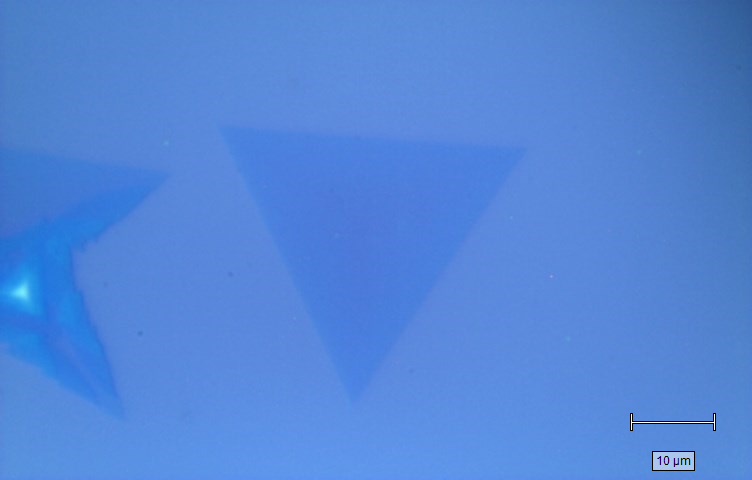
\includegraphics[scale=0.5]{WSe2/OMMap.png}
		\caption{An optical micrograph of the $WSe_2$ monolayer flake}
		\label{fig:WSe2OMMap}
	\end{center}
\end{figure}

These flakes have been characterized by PL and Raman spectroscopy (Figure \ref{fig:WSe2PLRamanSpectra}. A typical PL and Raman spectrum can be seen in Figure \ref{fig:WSe2PLRamanSpectra}. The peak is centred at 1.65 eV which suggest a monolayer nature of the flake (as the direct band gap of monolayer is 1.65 eV) and the peak appears mostly symmetrical with FWHM of 66 meV. The symmetry of the peak and the fact it can be fitted with a single function, suggest a negligible contribution from trions in contrast we what observed for $WS_2$  fakes. The Raman peak around 250 $cm^{-1}$ is a convolution of 2 peaks, an $E^1_{2g}$ and $A_{1g}$ vibrational modes, as already observed for bulk as well as exfoliated $WSe_2$.

\begin{figure}[H]
	\begin{center}
		\begin{subfigure}[b]{0.45\textwidth}
			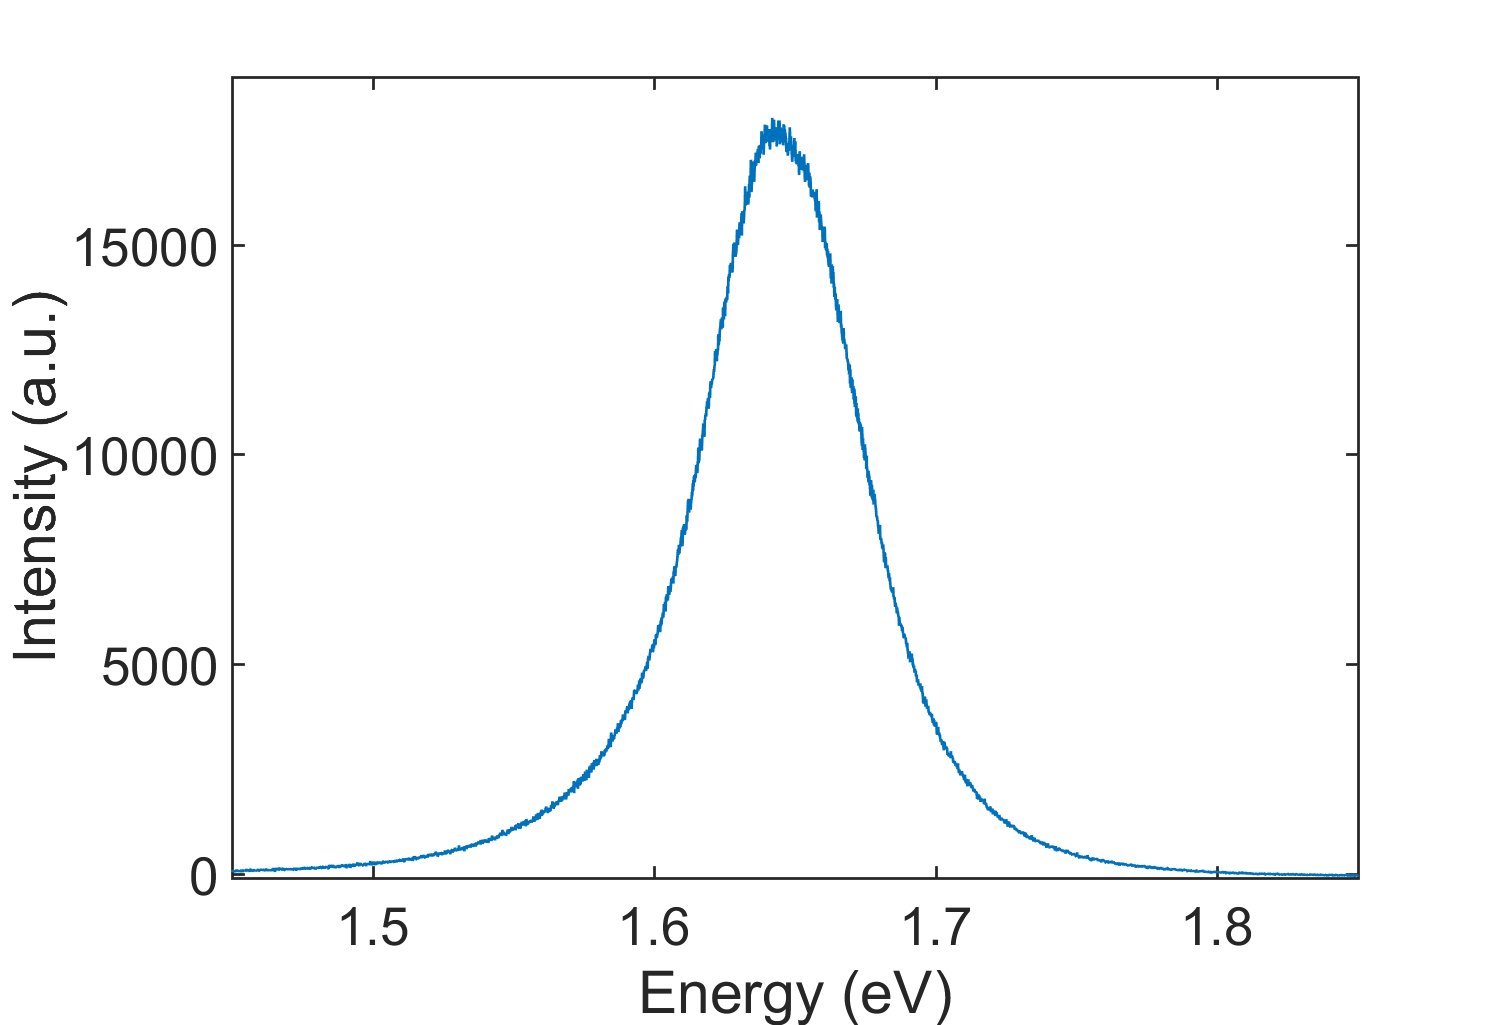
\includegraphics[width=\textwidth]{WSe2/PLSpectrum.png}
			\caption{Typical PL spectrum from monolayer $WSe_2$}
			\label{fig:WSe2PLSpectrum}
		\end{subfigure}
		\qquad
		\begin{subfigure}[b]{0.45\textwidth}
			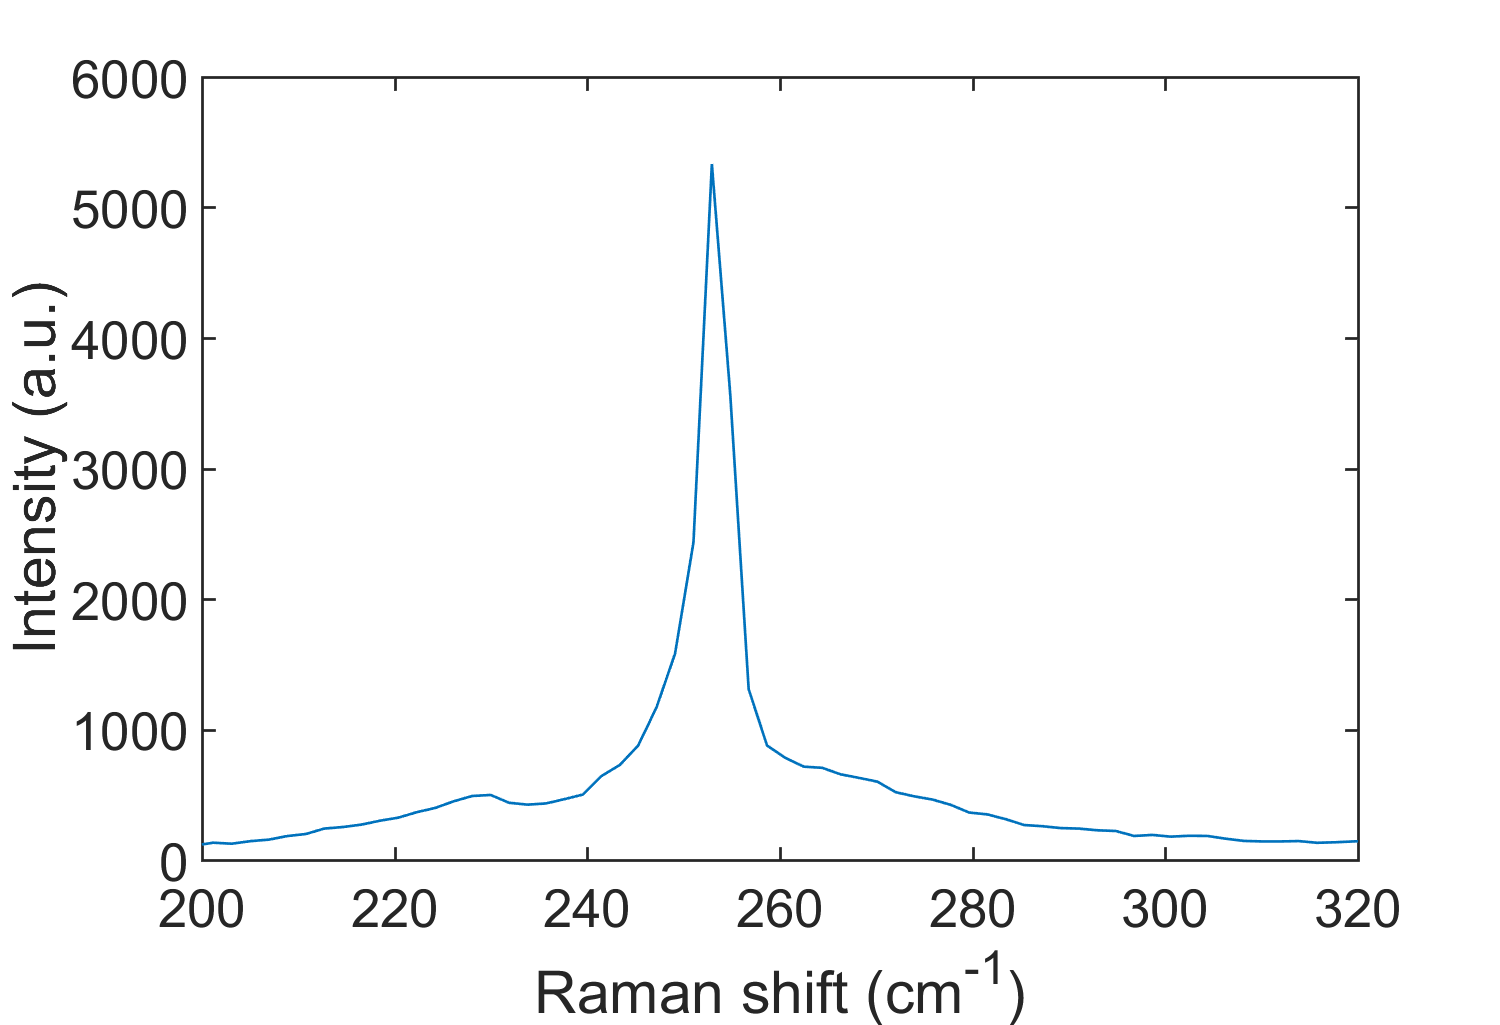
\includegraphics[width=\textwidth]{WSe2/RamanSpectrum.png}
			\caption{Typical Raman spectrum from monolayer $WSe_2$}
			\label{fig:WSe2RamanSpectrum}
		\end{subfigure}
		\caption{PL and Raman spectra from monolayer $WSe_2$}
		\label{fig:WSe2PLRamanSpectra}
	\end{center}
\end{figure}
	
\begin{figure}[H]
	\begin{center}
		\begin{subfigure}[b]{0.45\textwidth}
			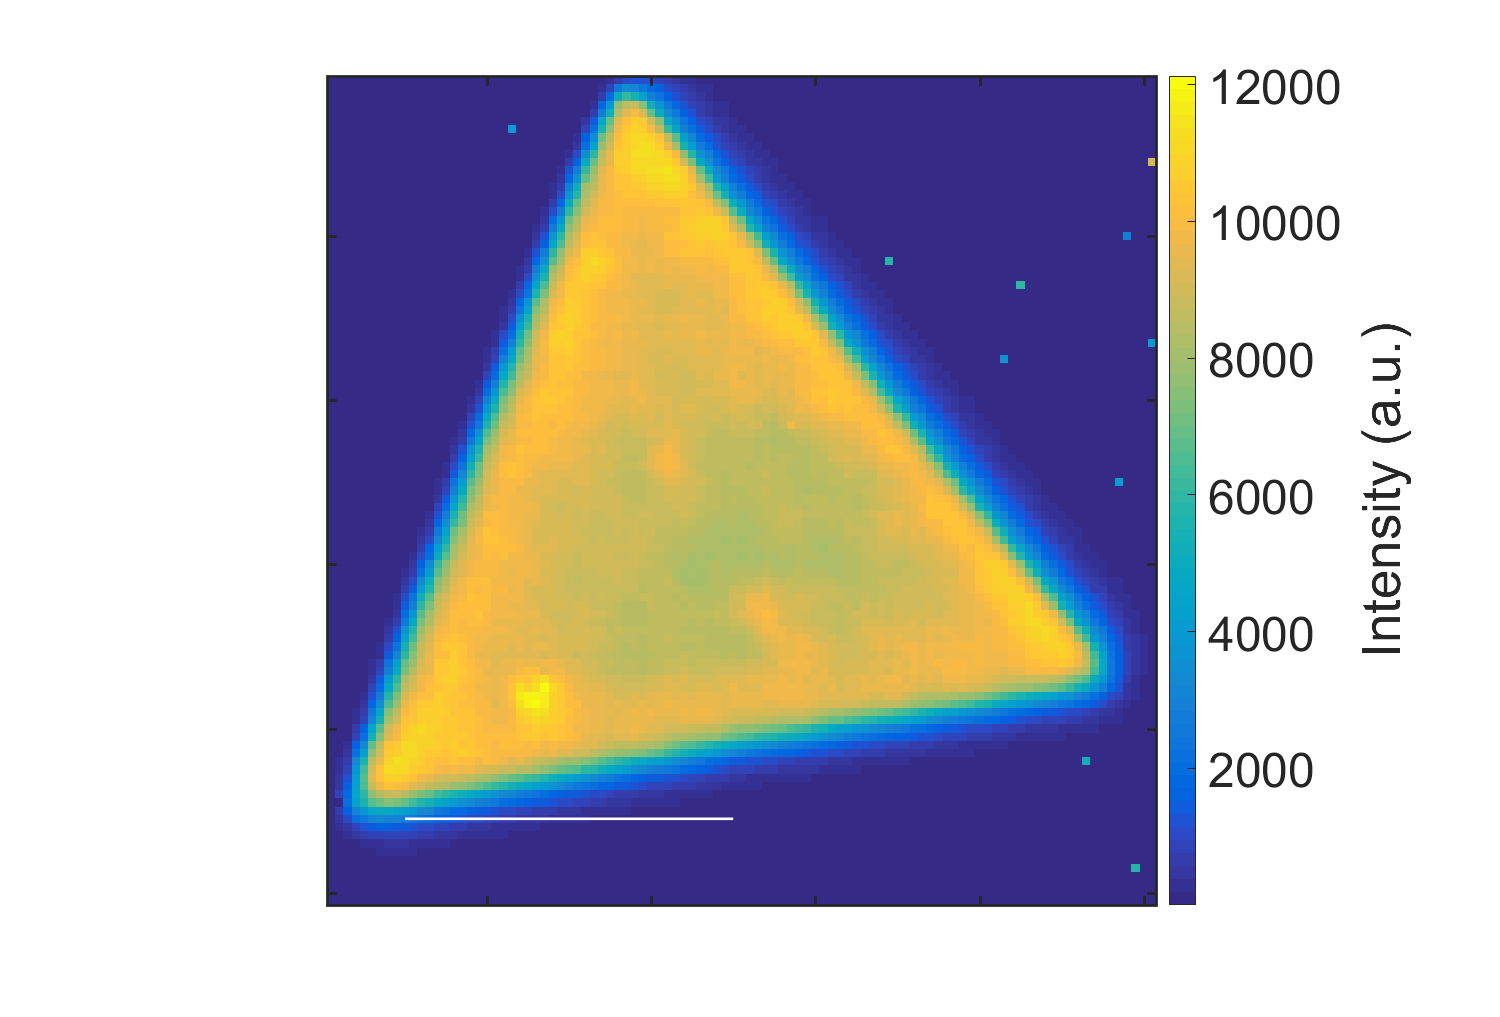
\includegraphics[width=\textwidth]{WSe2/PLIntensity.png}
			\caption{PL intensity}
			\label{fig:WSe2PLIntensityMap}
		\end{subfigure}
		\qquad
		\begin{subfigure}[b]{0.45\textwidth}
			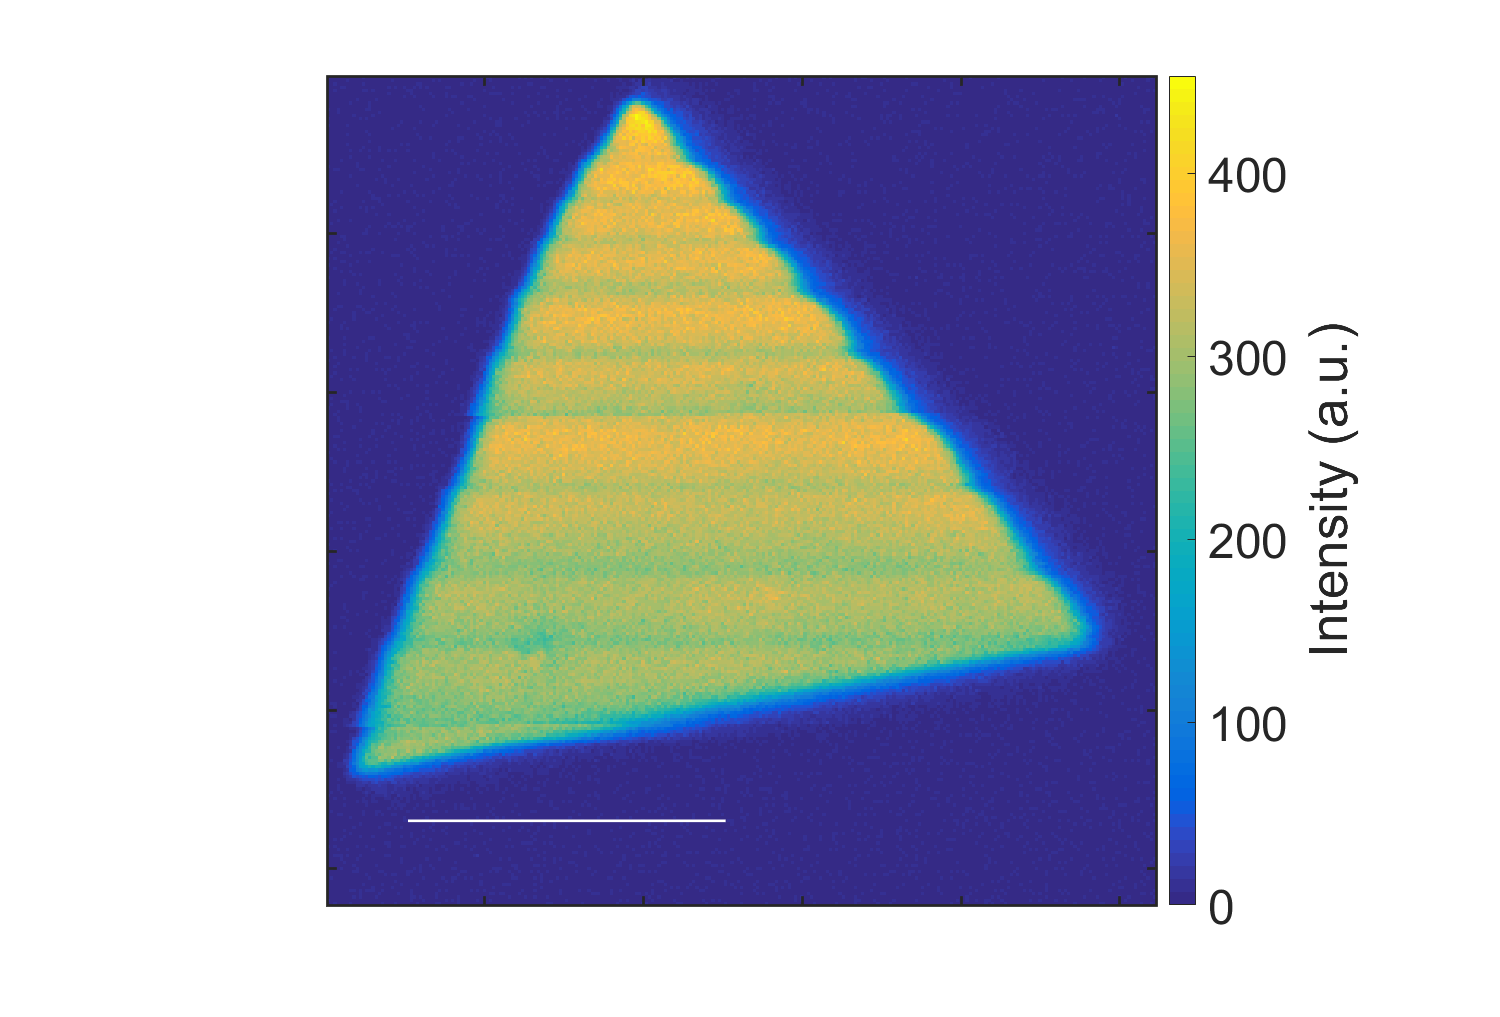
\includegraphics[width=\textwidth]{WSe2/RamanEIntensity.png}
			\caption{Raman $E^1_{2g}$ intensity}
		\end{subfigure}
		\caption{PL intensity and Raman $E^1_{2g}$ intensity maps}
	\end{center}
\end{figure}

A typical map of PL intensity of a $WSe_2$ sample can be seen in Figure \ref{fig:WSe2PLIntensityMap}. The PL intensity is homogeneous throughout the flake. It does not exhibit the trisecting pattern as seen in $WS_2$ samples e.g. Figure \ref{fig:WSe2PLIntensityMap}.
	
\begin{figure}[!h]
	\begin{center}
		\begin{subfigure}[b]{0.45\textwidth}
			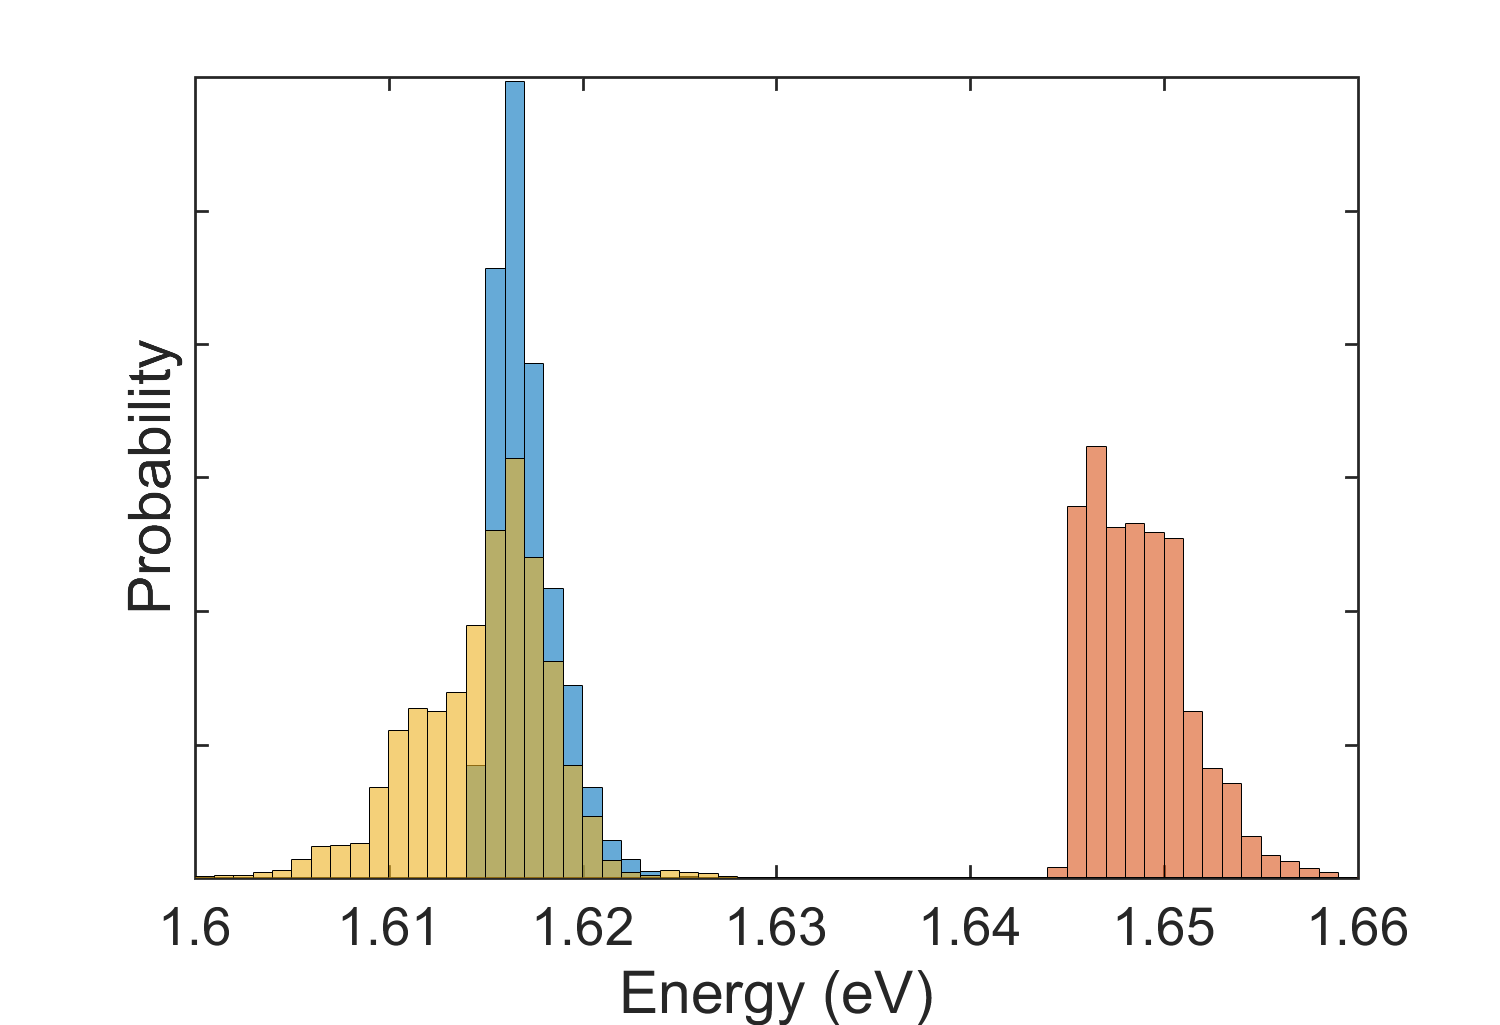
\includegraphics[width=\textwidth]{WSe2/WSe2PositionHistograms.png}
			\caption{WSe2 PL peak positions histograms}
			\label{fig:WSe2PLPositionHistograms}
		\end{subfigure}
		\qquad
		\begin{subfigure}[b]{0.45\textwidth}
			\includegraphics[width=\textwidth]{WSe2/Wse2WidthHistograms.png}
			\caption{WSe2 PL peak positions histograms}
			\label{fig:WSe2PLWidthHistograms}
		\end{subfigure}
		\caption{Comparison of PL peak positions and widths in different $WSe_2$ samples}
		\label{fig:WSe2PLHistograms}
	\end{center}
\end{figure}

A comparison of PL peak positions and widths between different samples of $WSe_2$ can be seen in Figure \ref{fig:WSe2PLHistograms}.

\begin{figure}[!h]
	\begin{center}
		\begin{subfigure}[b]{0.45\textwidth}
			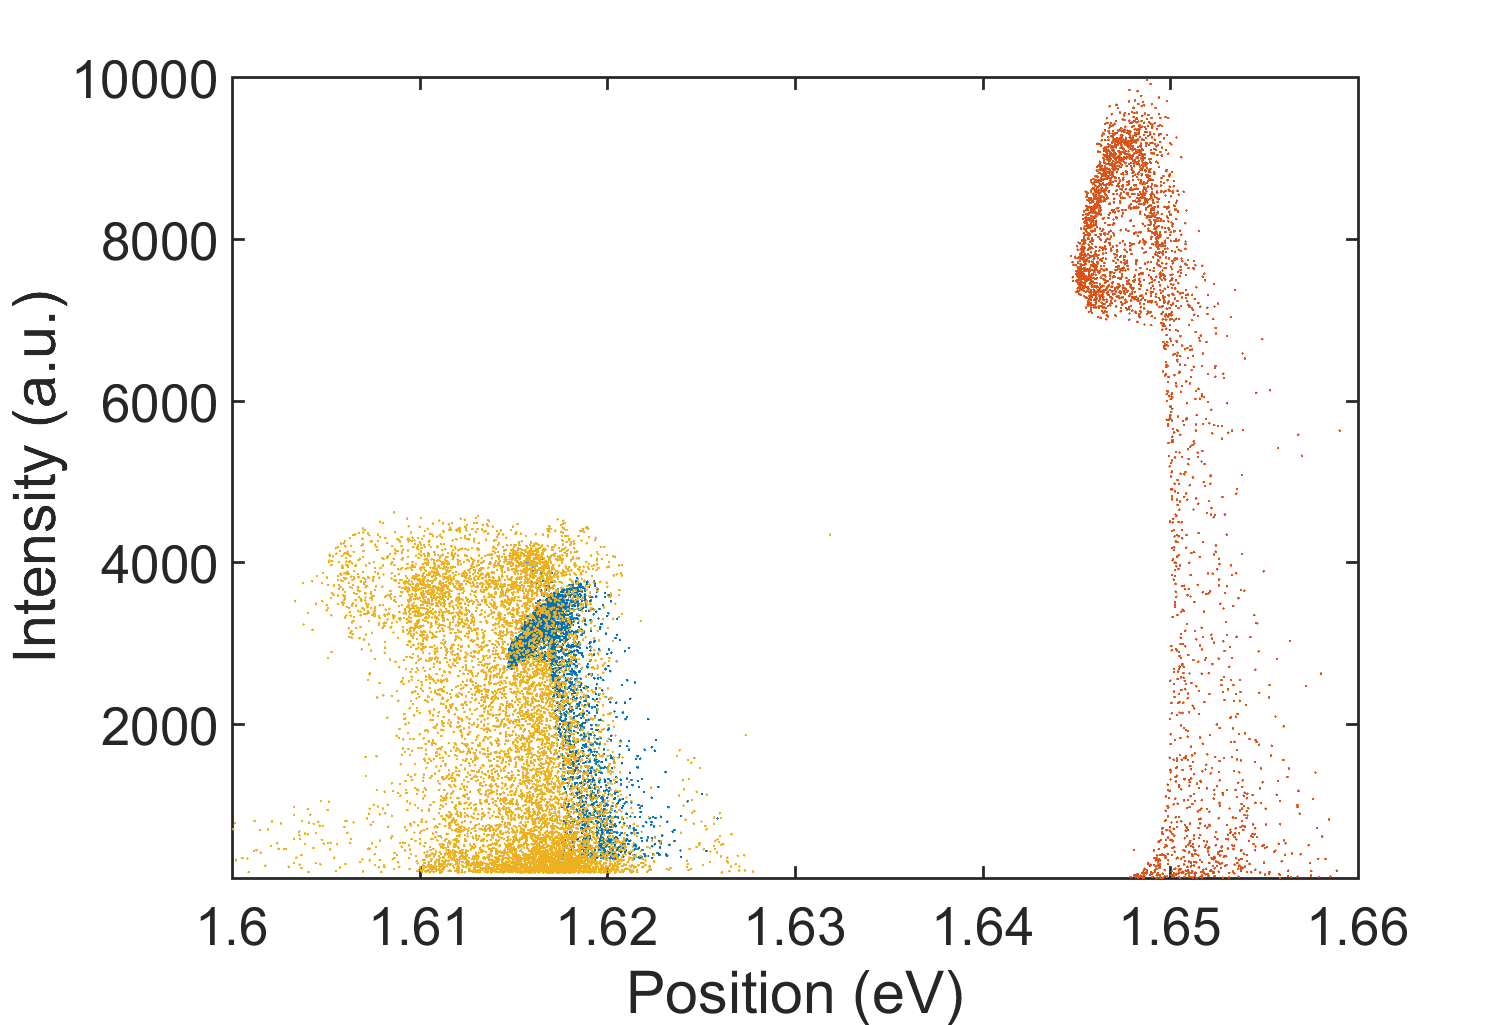
\includegraphics[width=\textwidth]{WSe2/WSe2PositionIntensityScatterComparison.png}
			\caption{Intensity vs position}
			\label{fig:WSe2PositionIntensityScatterComparison}
		\end{subfigure}
		\qquad
		\begin{subfigure}[b]{0.45\textwidth}
			\includegraphics[width=\textwidth]{WSe2/Wse2PositionWidthScatterComparison.png}
			\caption{Width vs position}
			\label{fig:WSe2PositionWidthScatterComparison}
		\end{subfigure}
		\caption{PL peak parameters distribution}
		\label{fig:WSe2ScatterComparison}
	\end{center}
\end{figure}

By plotting the intensity and width of the PL peaks against the peak position as seen in Figure \ref{fig:WSe2ScatterComparison} certain patterns can be observed. The intensity is mostly grouped around maximum values and relatively narrowly spread across the position spectrum. The thick flakes show much more even distribution of intensity across the position, which combined with the wide distribution of positions results in a much more inhomogeneous sample. The width and positions are generally well grouped with flakes with smaller width having more narrow distribution than those with greater width. Also few-layer flake shows a smaller peak width. Overall there is no obvious relation between position and width. 

%% Raman

The Raman spectroscopy is a very useful characterisation technique for TMDCs. For most TMDCs it can be used to identify the number of layers or strain within the layer. However in the case of $WSe_2$ the position of the $E^1_{2g}$ and $A_{1g}$ largely overlaps and therefore it is difficult to accurately determine the difference in their position. Because of that this method of identifying the number of layers cannot be employed easily. It is however still possible to examine the strain within the layers by noting the shift of the $E^1_{2g}$ peak. A Raman $E^1_{2g}$ peak position distribution from a representative sample can be seen in Figure \ref{fig:WSe2RamanPositionHistogram1}. The strain can be then determined from the mean position of $250.678 \pm 0.095$ $cm^{-1}$ to be 2.44 {\%} \cite{Dadgar2018}.

\begin{figure}[!h]
	\begin{center}
		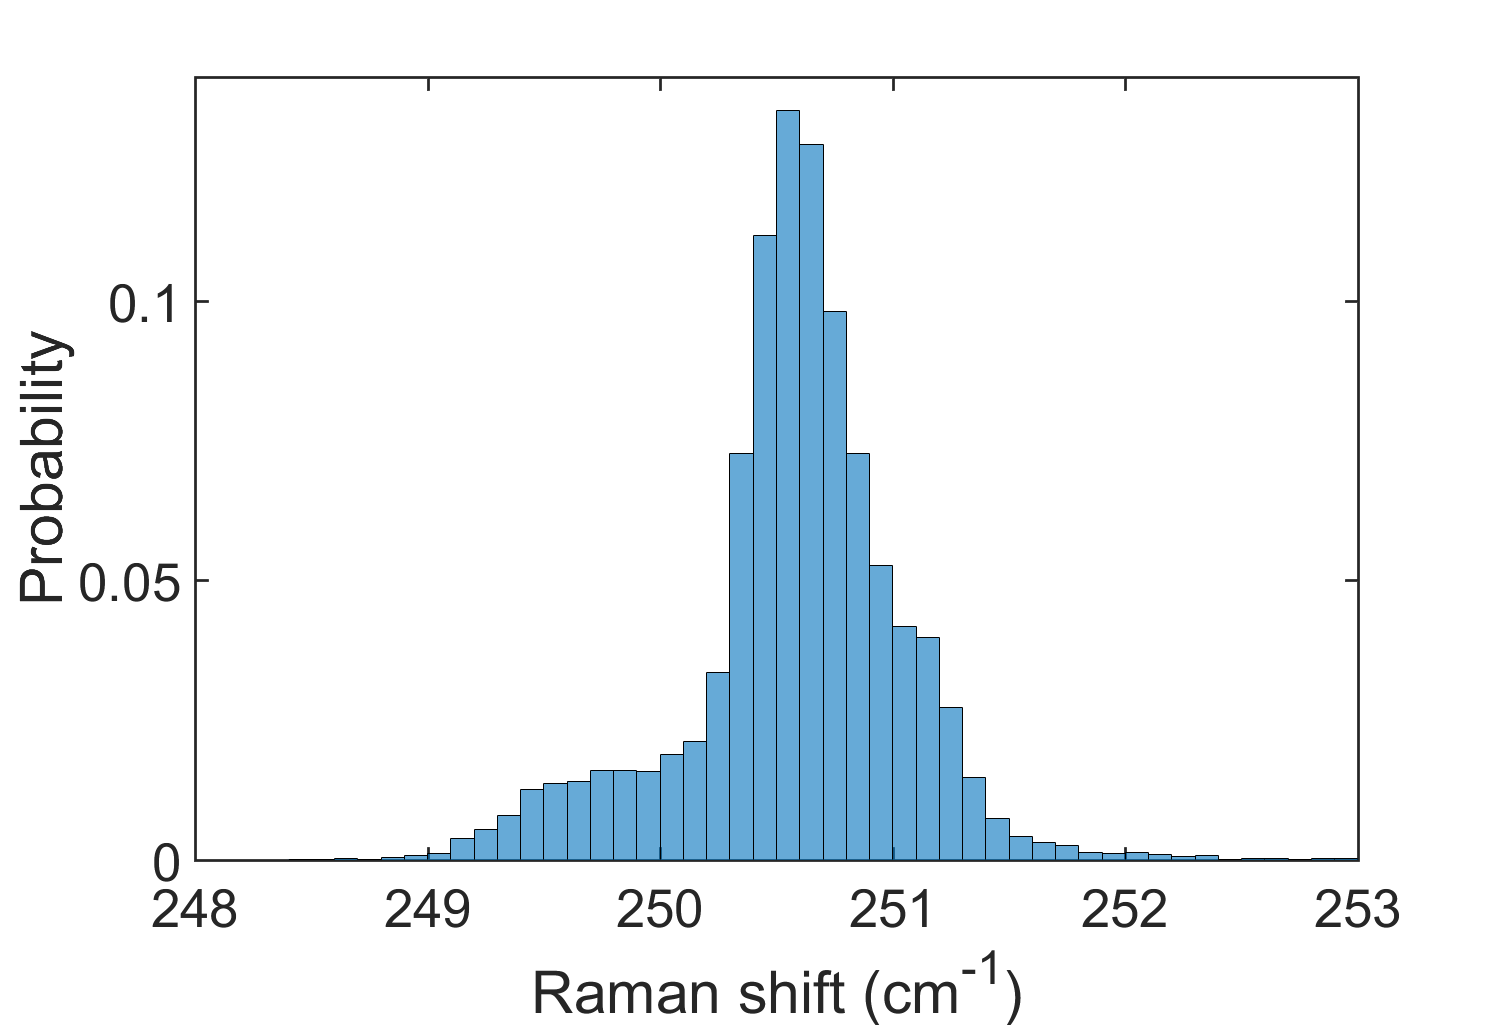
\includegraphics[scale=0.3]{WSe2/WSe2RamanPositionHistogram1.png}
		\caption{Histogram of Raman $E^1_{2g}$ peak position from monolayer $WSe_2$}
		\label{fig:WSe2RamanPositionHistogram1}
	\end{center}
\end{figure}

\begin{figure}[!h]
	\begin{center}
		\begin{subfigure}[b]{0.4\textwidth}
			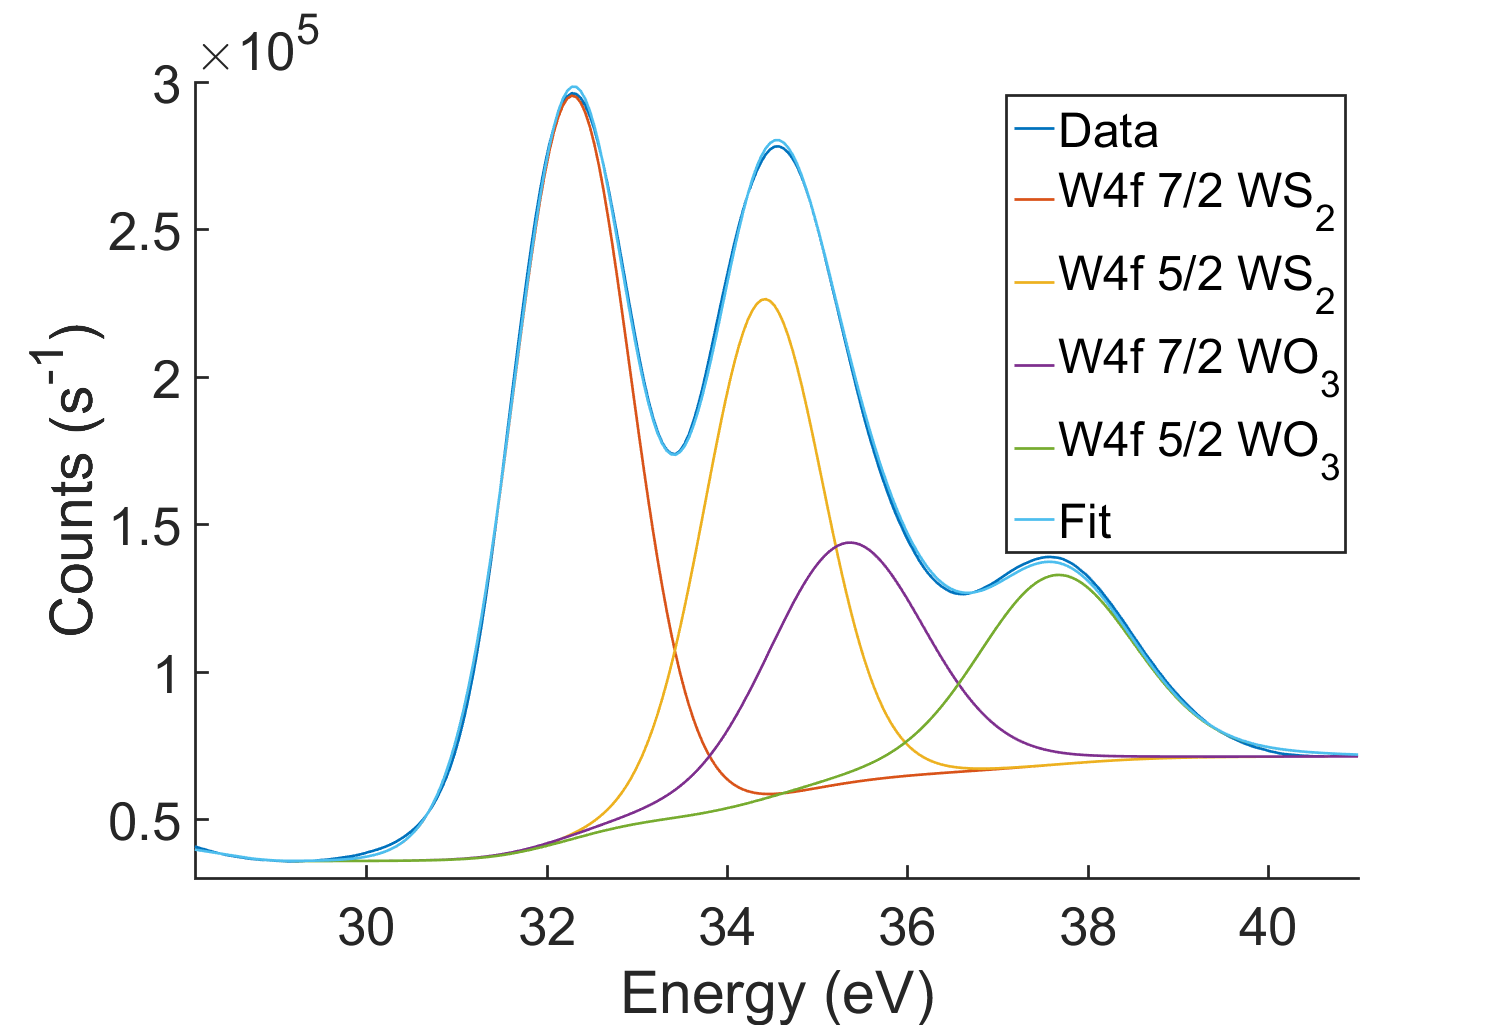
\includegraphics[width=\textwidth]{WSe2/XPSW4fThin.png}
			\caption{Thin flakes}
			\label{fig:WSe2XPSThinW}
		\end{subfigure}
		\qquad
		\begin{subfigure}[b]{0.4\textwidth}
			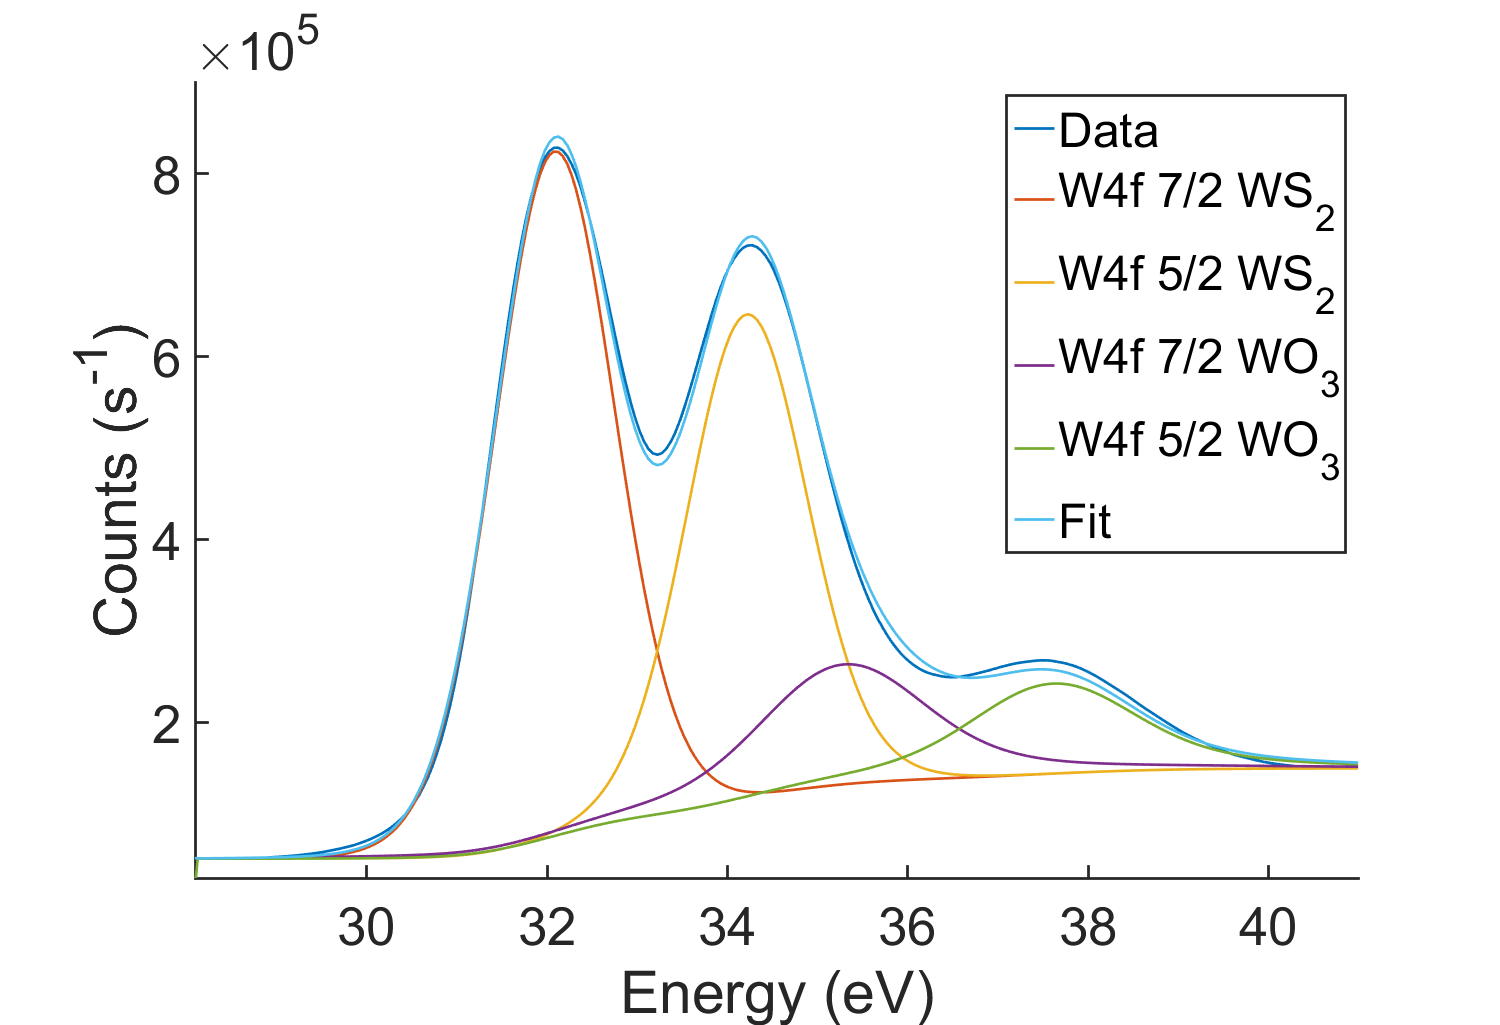
\includegraphics[width=\textwidth]{WSe2/XPSW4fThick.png}
			\caption{Thick flakes}
			\label{fig:WSe2XPSThickW}
		\end{subfigure}
		
		\begin{subfigure}[b]{0.4\textwidth}
			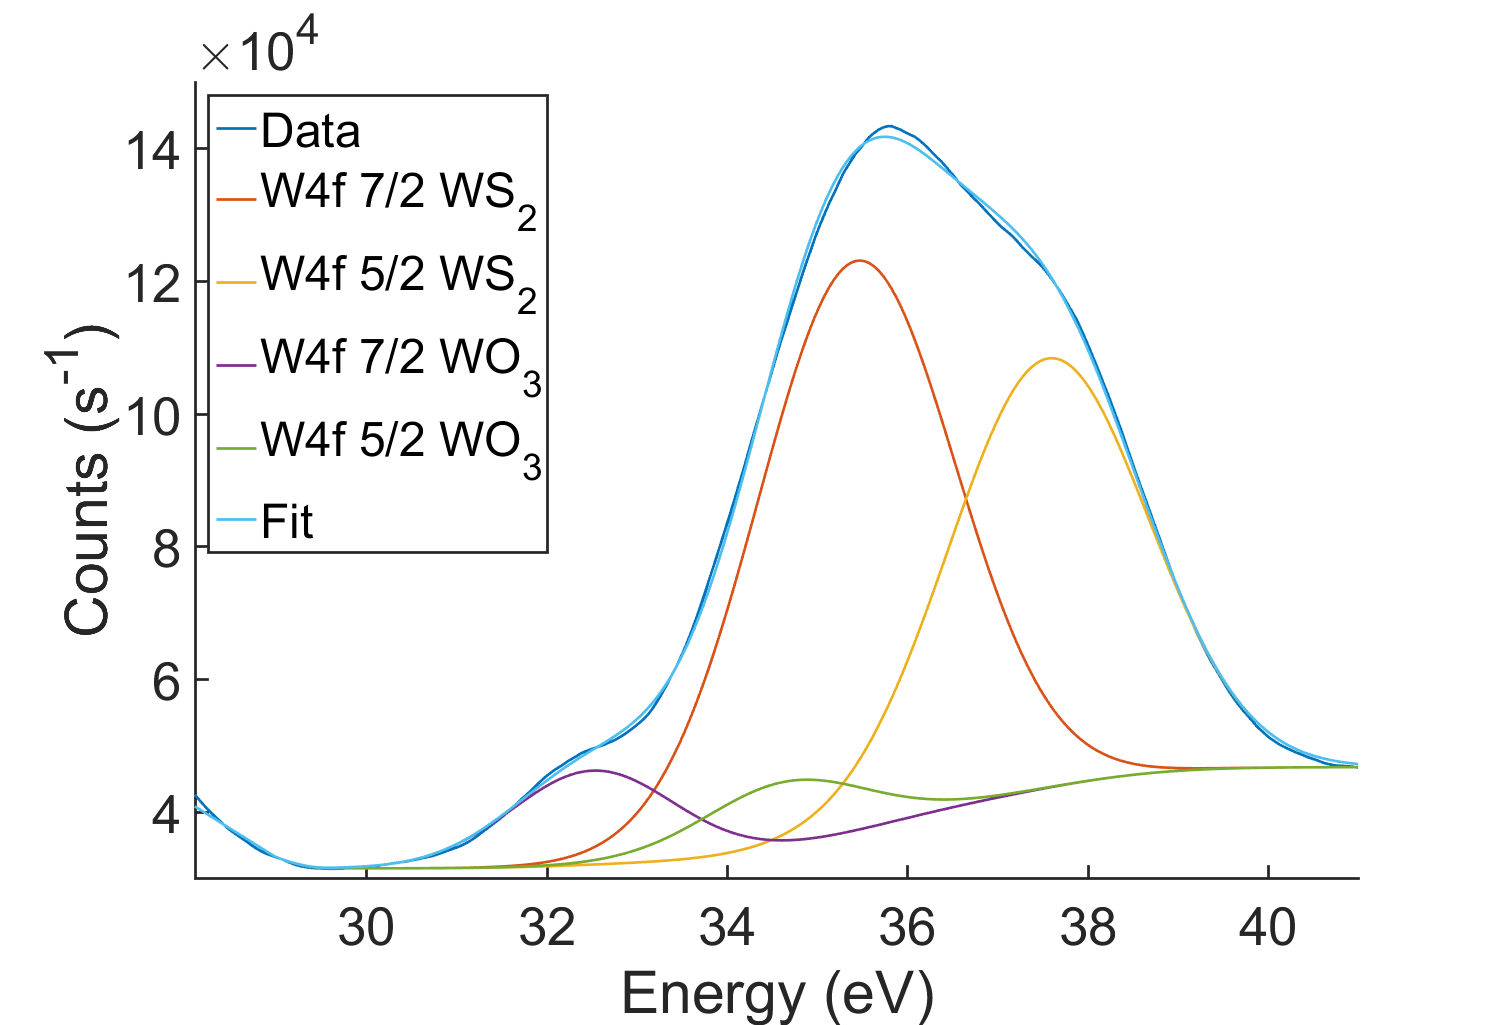
\includegraphics[width=\textwidth]{WSe2/XPSW4fRef.png}
			\caption{Empty area}
			\label{fig:WSe2XPSRefW}
		\end{subfigure}
		\caption{XPS spectra of W4f peaks in different areas of the sample}
		\label{fig:WSe2XPSW}
	\end{center}
\end{figure}

\begin{figure}[!h]
	\begin{center}
		\begin{subfigure}[b]{0.4\textwidth}
			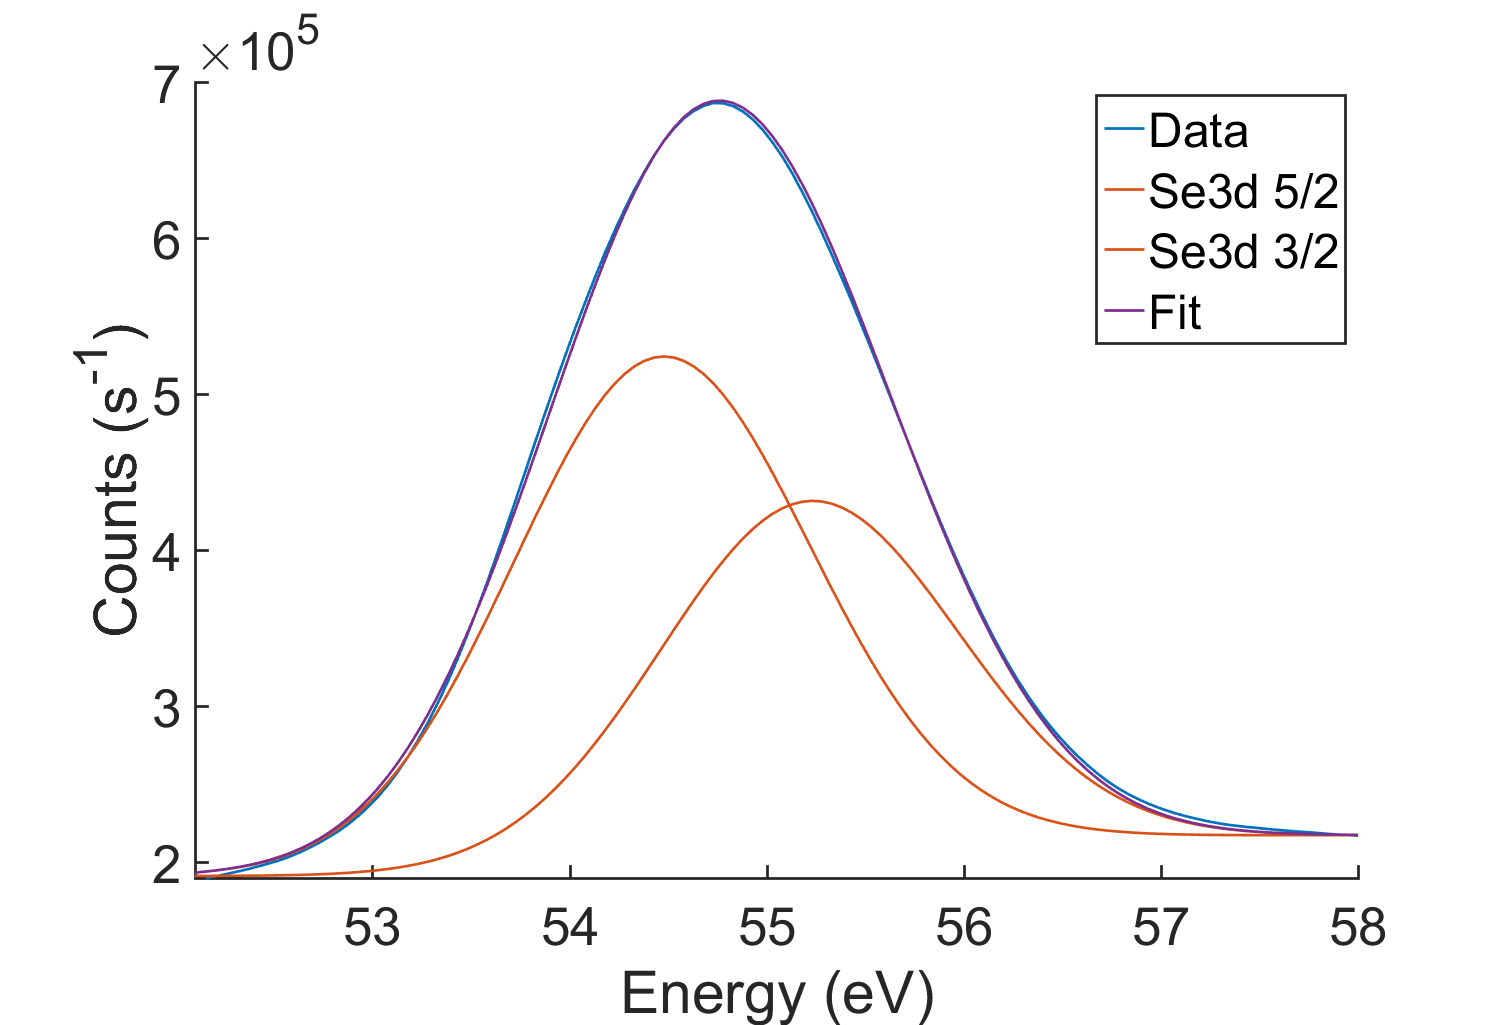
\includegraphics[width=\textwidth]{WSe2/XPSSe3dThin.png}
			\caption{Thin flakes}
			\label{fig:WSe2XPSThinSe}
		\end{subfigure}
		\qquad
		\begin{subfigure}[b]{0.4\textwidth}
			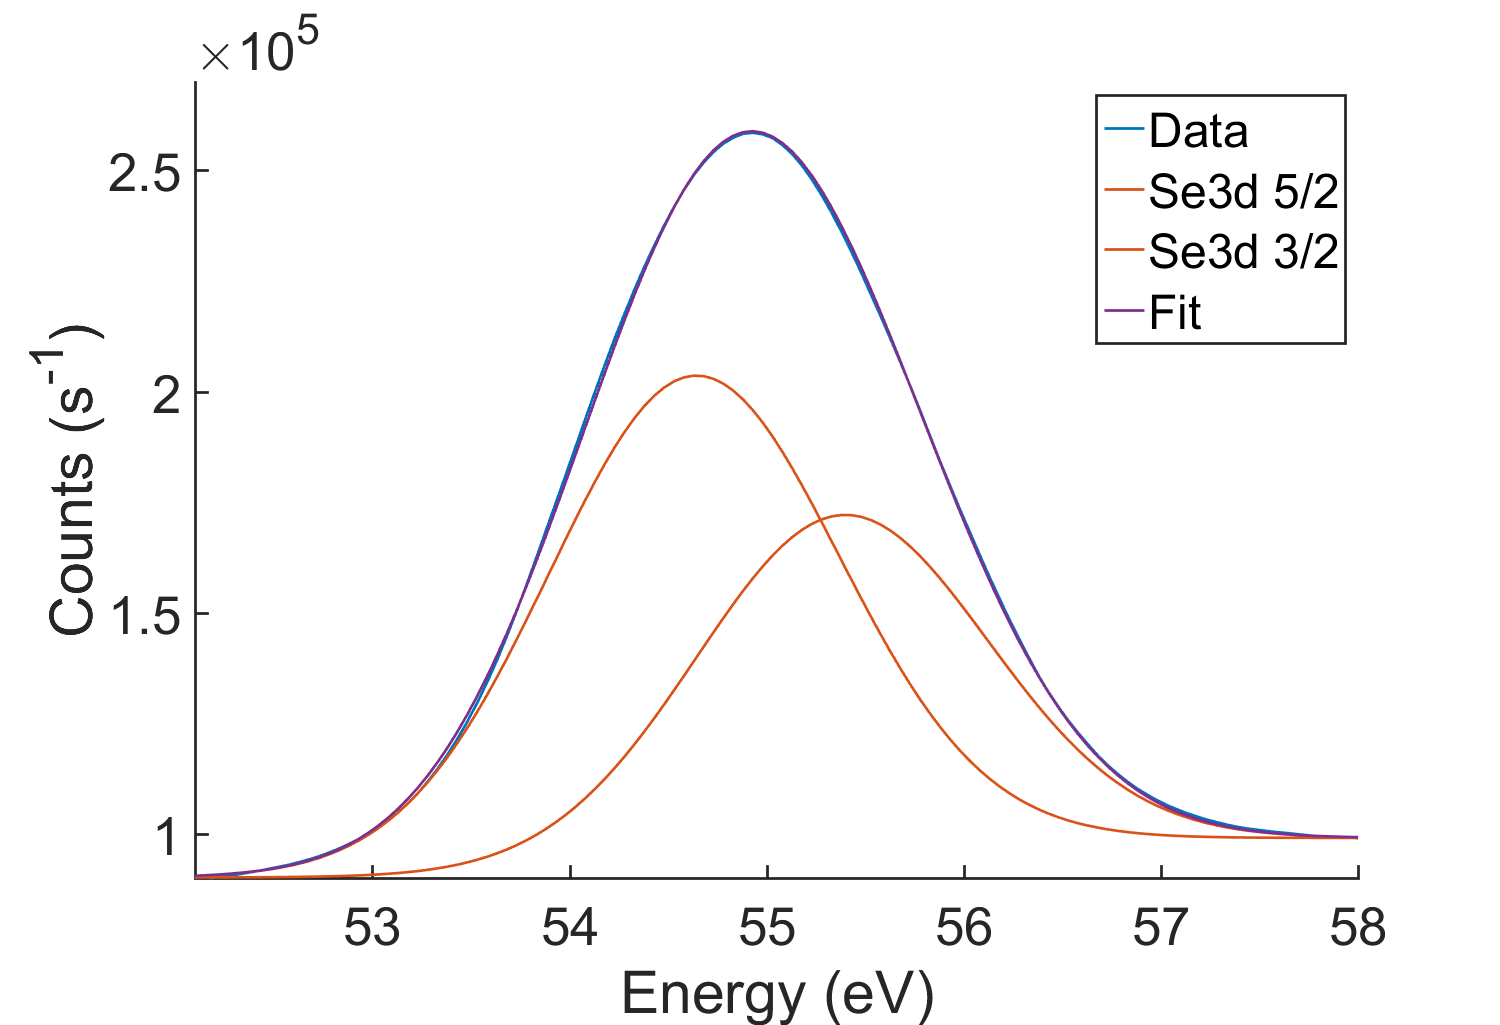
\includegraphics[width=\textwidth]{WSe2/XPSSe3dThick.png}
			\caption{Thick flakes}
			\label{fig:WSe2XPSThickSe}
		\end{subfigure}
		
		\begin{subfigure}[b]{0.4\textwidth}
			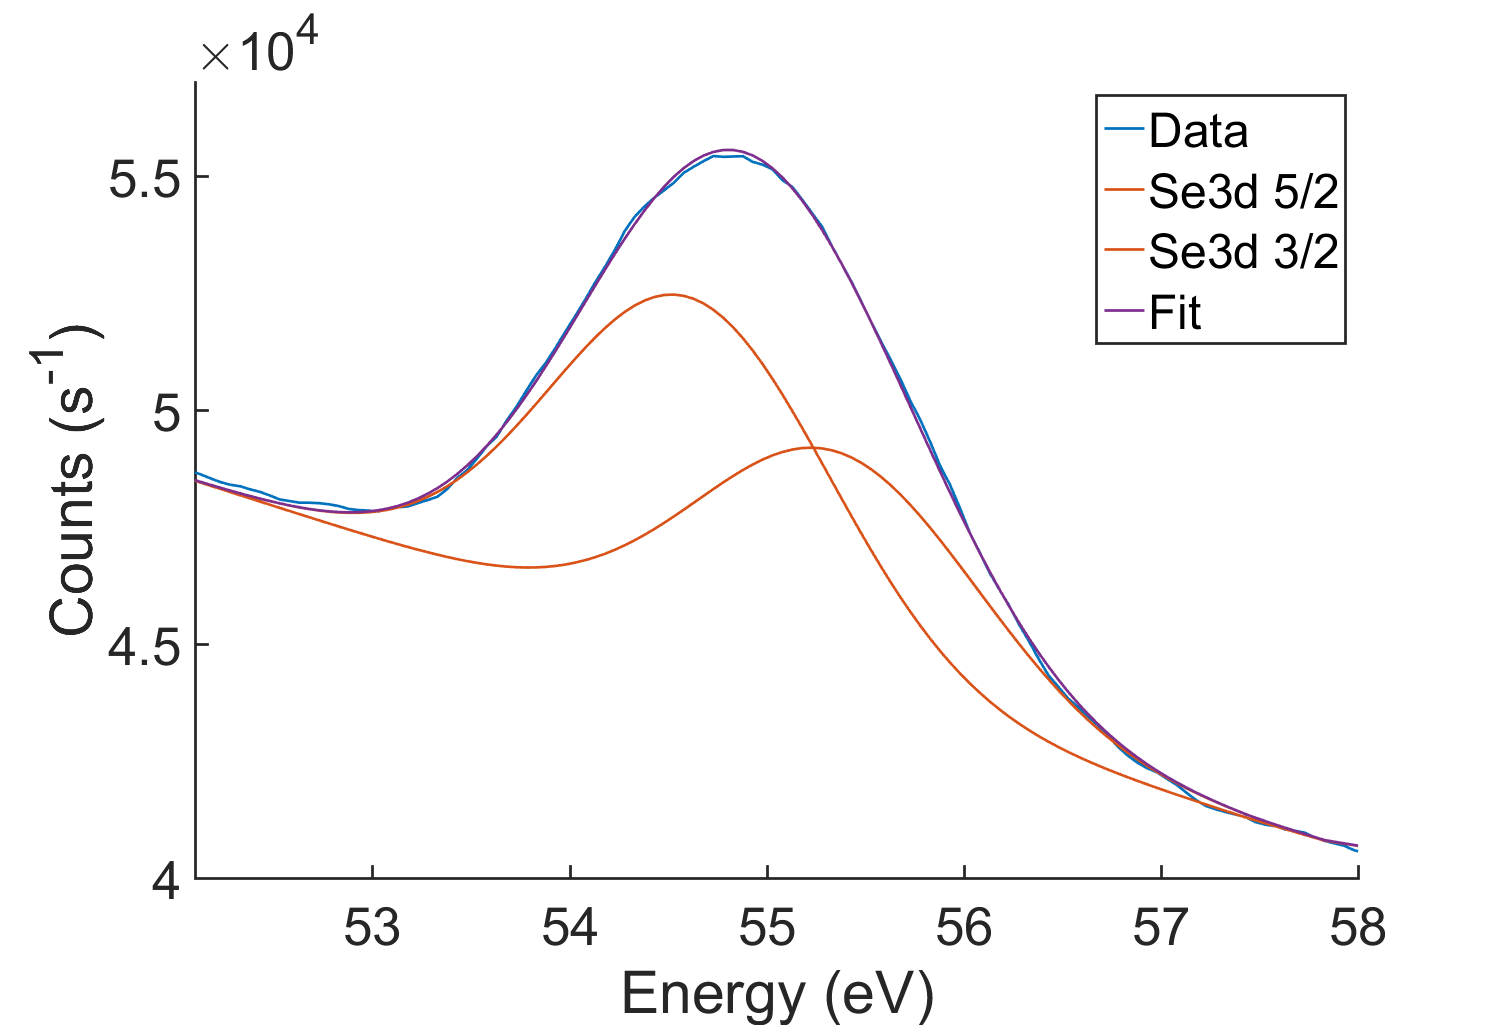
\includegraphics[width=\textwidth]{WSe2/XPSSe3dRef.png}
			\caption{Empty area}
			\label{fig:WSe2XPSRefSe}
		\end{subfigure}
		\caption{XPS spectra of Se3d peaks in different areas of the sample}
		\label{fig:WSe2XPSSe}
	\end{center}
\end{figure}

\begin{figure}[!h]
	\begin{center}
		\begin{subfigure}[b]{0.4\textwidth}
			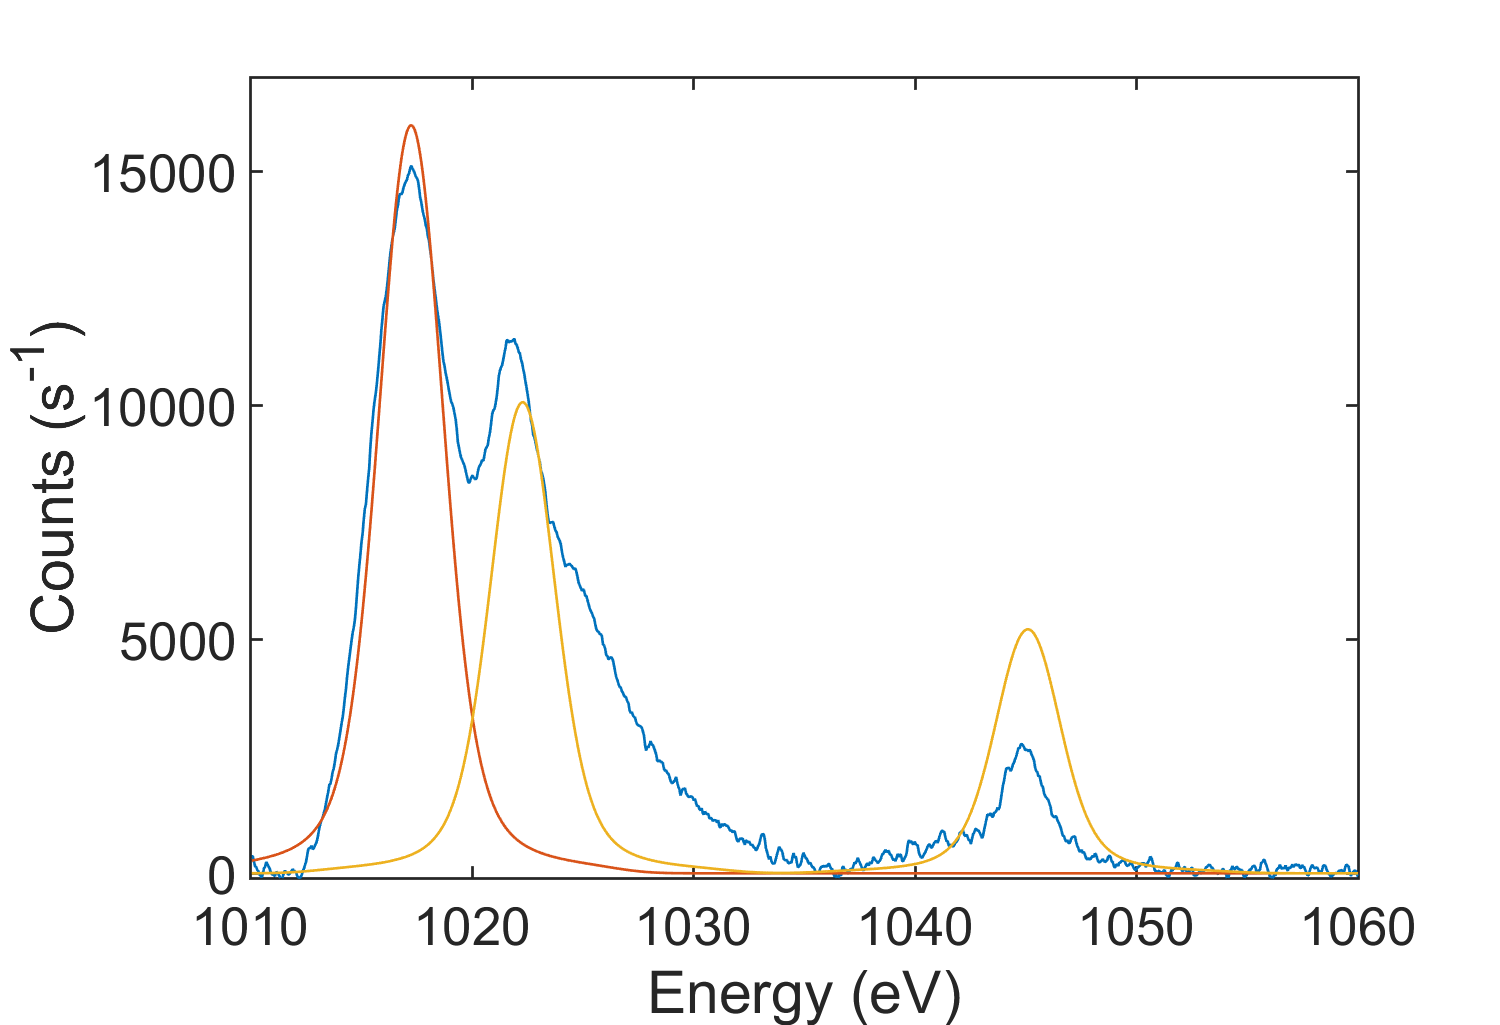
\includegraphics[width=\textwidth]{WSe2/WSe2XPSThinZn.png}
			\caption{Thin flakes}
			\label{fig:WSe2XPSThinZn}
		\end{subfigure}
		\qquad
		\begin{subfigure}[b]{0.4\textwidth}
			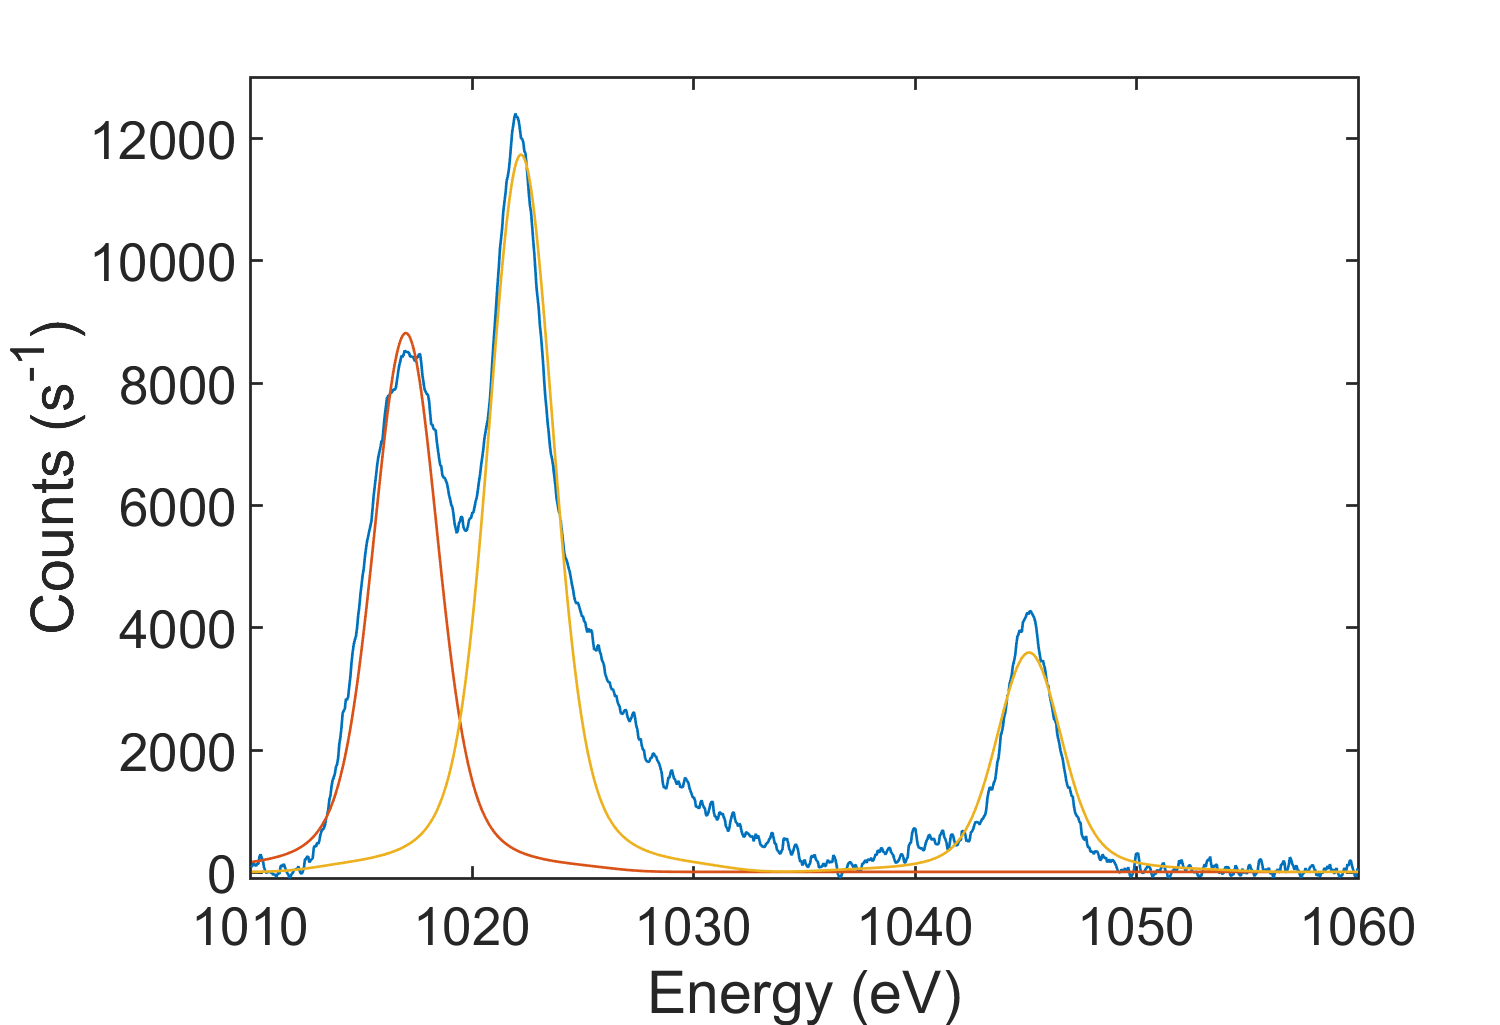
\includegraphics[width=\textwidth]{WSe2/WSe2XPSThickZn.png}
			\caption{Thick flakes}
			\label{fig:WSe2XPSThickZn}
		\end{subfigure}
		
		\begin{subfigure}[b]{0.4\textwidth}
			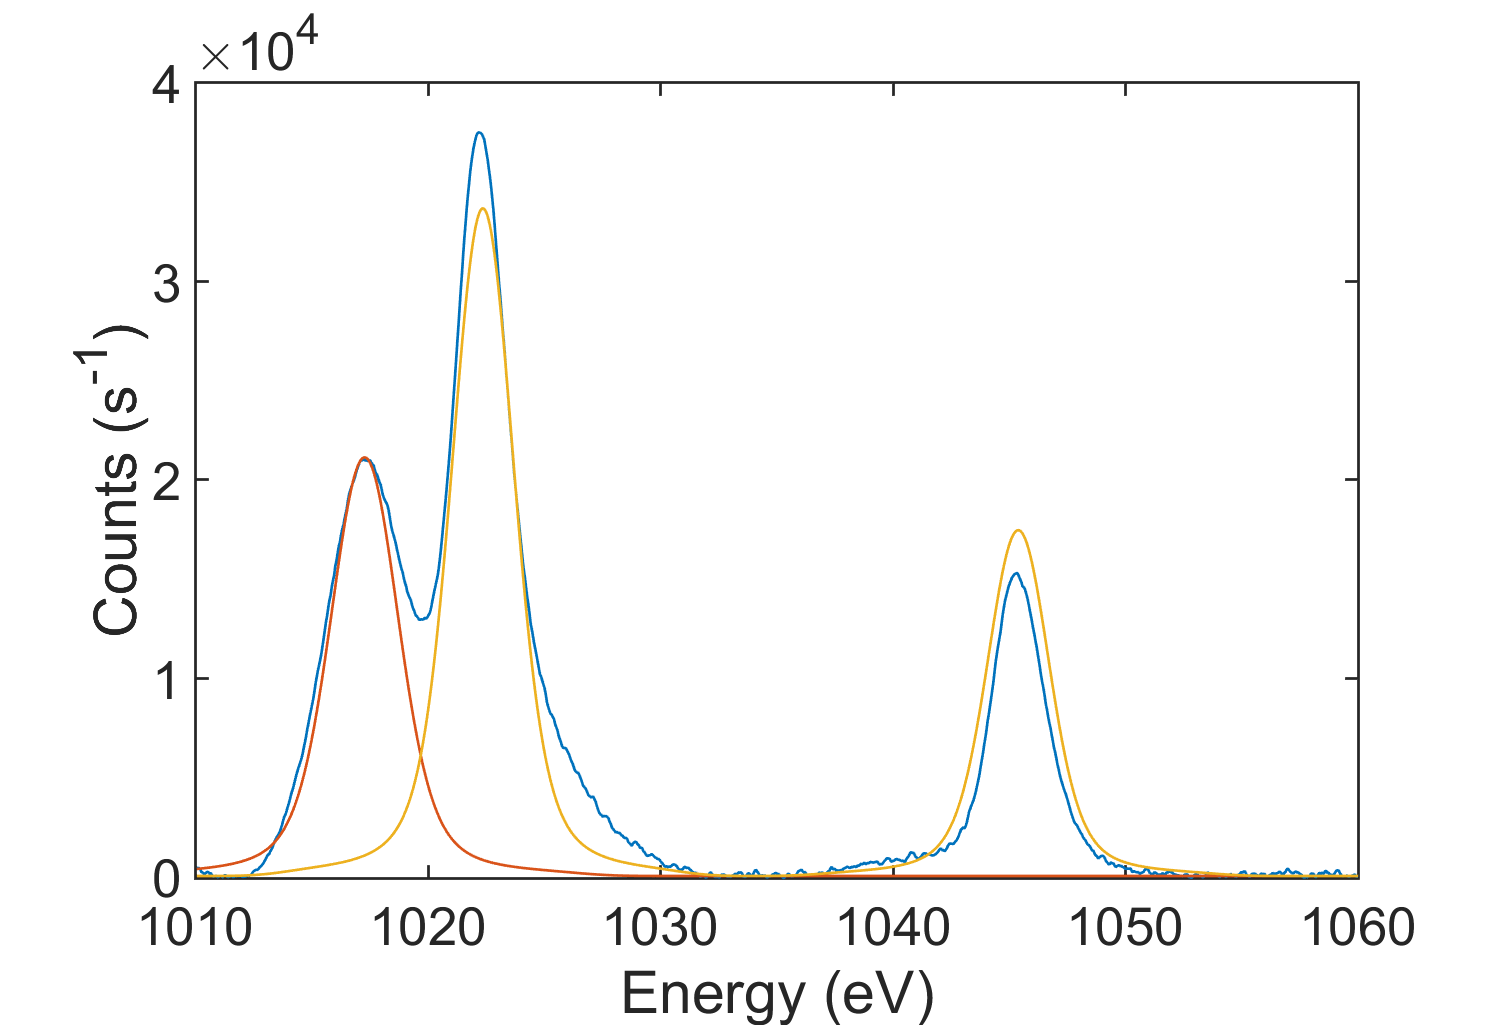
\includegraphics[width=\textwidth]{WSe2/WSe2XPSRefZn.png}
			\caption{Empty area}
			\label{fig:WSe2XPSRefZn}
		\end{subfigure}
		\caption{XPS spectra of Zn2p peaks in different areas of the sample}
		\label{fig:WSe2XPSZn}
	\end{center}
\end{figure}

The sample has been further characterised with XPS. Three areas were selected for measurements, one with thin, mono or double layer $WSe_2$, one with thick bulk $WSe_2$ and one with no visible $WSe_2$ flakes. The Figure \ref{fig:WSe2XPSW} shows W4f core levels measured in those spots. The first area (Figure \ref{fig:WSe2XPSThinW}), with thin flake shows one doublet at 32.08 eV and 34.23 eV and a second doublet at 35.33 eV and 37.68 eV. The first doublet corresponds to $WSe_2$ while the second one can be attributed to $WO_3$. Since the spot size in the measurement covers both the flake as well as some surrounding substrate it is possible that the $WO_3$ is located outside of the flake. Furthermore the background indicates that the emission from $WSe_2$ came from surface and therefore the $WSe_2$ flake is not contaminated with $WO_3$. 
The second area with thicker flakes (Figure \ref{fig:WSe2XPSThickW}) shows similarly two doublets: one at 32.28 eV and 34.43 eV and a second one at 35.38 eV and 37.63 eV. Similarly to the thin area with thin flake we can ascribe the former to the $WSe_2$ and the latter to $WO_3$. There is a small shift of 0.2 eV between $WSe_2$ from the thin flake and $WSe_2$ from the thick flake. It is possible that XPS is sensitive to the number of layers in $WSe_2$ and TMDCs in general since it is known that number of layers does modify the electronic structure of the material. The $WO_3$ is found to be at the same position in both areas. The $WO_3$ peak is also relatively weaker in the area with the thick flake than in the area with thin flake which could be a result of the thick flake having larger surface area than the thin flake and smaller presence of $WO_3$ around the flake. 
Additionally an empty area (Figure \ref{fig:WSe2XPSRefW}) with no visible flakes has been measured. Similarly two doublets, one at 32.58 eV and 34.73 eV and a second one at 35.48 eV and 37.58 eV have been fitted and their presence can be again explained by presence of $WSe_2$ and $WO_3$. The $WSe_2$ peak is shifted in relation to that from the thin flake by 0.5 eV which could indicate presence of a highly defective $WS_2$ or very small amounts of very bulk $WS_2$. The $WS_2$ peak is also much weaker than that of the $WO_3$ which is expected since there is no visible $WS_2$. This result suggesting presence of residues of tungsten oxide species across the whole substrate and thus also possibly across the grown flakes of $WSe_2$. This result corroborates the evidence of chemical purity of $WSe_2$.

We can also look at Se3d core levels measured at the same locations. As seen in Figure \ref{fig:WSe2XPSThinSe}, taken from an area with the thin flake, we can fit it with one doublet corresponding to the presence of $WSe_2$ at 54.48 eV and 55.23 eV. Similarly in Figure \ref{fig:WSe2XPSThickSe} we can see Se3d peaks taken from area with the thick flake and can fit it with a doublet at 54.63 eV and 55.38 eV which also corresponds to the $WSe_2$. Similar to the W4f levels there is a shift of 0.15 eV between those two flakes which can be explained by their thickness which changes the electronic structure. The Se3d levels measured in the reference empty area also can be fitted with a doublet at 54.53 eV and 55.33 eV which can be attributed to $WSe_2$. Similarly there is a shift of 0.05 eV from the peak associated with the thin flake, which is much smaller than the W4f peak shift. The Se3d peak from the empty area is about a magnitude weaker than that from either the thin or thick flake which is expected as no visible flake was observed. It does however indicate a non insignificant presence of $WSe_2$, perhaps in the form of nuclei that never grew into proper flakes or flakes that shrunk or became etched and are highly defective and thinner than monolayer. The Se3d from the empty area also exhibits a steep background which indicates that the Se is covered with some layer, perhaps that of $WO_3$. 

Finally the Zn2p levels were measured across the same areas. As seen in Figure \ref{fig:WSe2XPSThinZn} a doublet can be identified at 1022.02 eV and 1045.11 eV together with a single peak at 1017.33 eV taken from a thin flake. Similarly in Figure \ref{fig:WSe2XPSThickZn} the doublet is located at 1022.23 eV and 1045.16 eV and a single peak at 1017.03 eV. The reference area shows a doublet at 1045.39 eV and 1022.38 eV and a single peak at 1017.29 eV. It seems therefore that the peak position of the Zn2p doublet does not changes significantly from the empty reference area and the thin or thick flake. The peak intensity in the empty area is also much greater than that of the peak in the area with thin or thick flakes. It suggests then that the Zn that was used in the synthesis is therefore located mostly on a substrate and not on the $WSe_2$ flakes.

\section{Conclusions}

In this chapter I have presented and discussed the electronic band structure and the physical characterization of CVD grown 2H $WSe_2$.
The CVD synthesis of $WSe_2$ is quite challenging and not much work has been reported so far in the literature due to the low reactivity of Se. We have concluded that the grown material is pure, and possibly have high crystallinity as demonstrated from the relatively small FWHM of the PL peak. Additionally, thanks to micrometric lateral size resolution of the XPS analysis we could distinguish and parameterise the difference in binding energy of W 4f orbitals as a function of the thickness of the flakes for the first time. Furthermore, we could prove that a small amount of $WO_3$ is spread all over the substrate and it is not chemically bound to $WSe_2$. Similarly, it was interesting to observe the presence of elemental Se on the bare substrates. In contrast with the belief that the sticking coefficient of chalcogen elements is very low as compared to metals such as W and Mo, this evidence can shed light into the growth mechanism via CVD of atomically thin materials.